%%%%%%%%%%%%%%%%%%%%%%%%%%%%%%%%%%%%%%%%%
% Beamer Presentation
% LaTeX Template
% Version 1.0 (10/11/12)
%
% This template has been downloaded from:
% http://www.LaTeXTemplates.com
%
% License:
% CC BY-NC-SA 3.0 (http://creativecommons.org/licenses/by-nc-sa/3.0/)
%
%%%%%%%%%%%%%%%%%%%%%%%%%%%%%%%%%%%%%%%%%

%----------------------------------------------------------------------------------------
%	PACKAGES AND THEMES
%----------------------------------------------------------------------------------------

\documentclass{beamer}

\mode<presentation> {

% The Beamer class comes with a number of default slide themes
% which change the colors and layouts of slides. Below this is a list
% of all the themes, uncomment each in turn to see what they look like.

%\usetheme{default}
%\usetheme{AnnArbor}
%\usetheme{Antibes}
%\usetheme{Bergen}
%\usetheme{Berkeley}
\usetheme{Berlin}
%\usetheme{Boadilla}
%\usetheme{CambridgeUS}
%\usetheme{Copenhagen}
%\usetheme{Darmstadt}
%\usetheme{Dresden}
%\usetheme{Frankfurt}
%\usetheme{Goettingen}
%\usetheme{Hannover}
%\usetheme{Ilmenau}
%\usetheme{JuanLesPins}
%\usetheme{Luebeck}
%\usetheme{Madrid}
%\usetheme{Malmoe}
%\usetheme{Marburg}
%\usetheme{Montpellier}
%\usetheme{PaloAlto}
%\usetheme{Pittsburgh}
%\usetheme{Rochester}
%\usetheme{Singapore}
%\usetheme{Szeged}
%\usetheme{Warsaw}

% As well as themes, the Beamer class has a number of color themes
% for any slide theme. Uncomment each of these in turn to see how it
% changes the colors of your current slide theme.

%\usecolortheme{albatross}
\usecolortheme{beaver}
%\usecolortheme{beetle}
%\usecolortheme{crane}
%\usecolortheme{dolphin}
%\usecolortheme{dove}
%\usecolortheme{fly}
%\usecolortheme{lily}
%\usecolortheme{orchid}
%\usecolortheme{rose}
%\usecolortheme{seagull}
%\usecolortheme{seahorse}
%\usecolortheme{whale}
%\usecolortheme{wolverine}

%\setbeamertemplate{footline} % To remove the footer line in all slides uncomment this line
%\setbeamertemplate{footline}[page number] % To replace the footer line in all slides with a simple slide count uncomment this line

%\setbeamertemplate{navigation symbols}{} % To remove the navigation symbols from the bottom of all slides uncomment this line
}

% math definition
\newcommand{\indep}{\mathrel{\text{\scalebox{1.07}{$\perp\mkern-10mu\perp$}}}}


%
\usepackage{graphicx} % Allows including images
\usepackage{booktabs} % Allows the use of \toprule, \midrule and \bottomrule in tables
\usepackage{comment}

%macros from Bob Gray
\usepackage{"./macro/GrandMacros"}
\usepackage{"./macro/Macro_BIO235"}

\usepackage[normalem]{ulem}

% tikz
\usepackage{tikz}
\usetikzlibrary{bayesnet}


%----------------------------------------------------------------------------------------
%	TITLE PAGE
%----------------------------------------------------------------------------------------

\title[HDP-HMM-SLDS]{Hierarchical Dirichlet Process for Switching Linear Dynamical Systems} % The short title appears at the bottom of every slide, the full title is only on the title page

\author{Will Townes, Jeremiah Zhe Liu} % Your name

\date{\today} % Date, can be changed to a custom date

\begin{document}

\begin{frame}
\titlepage % Print the title page as the first slide
\end{frame}

\begin{frame}
\frametitle{Overview} % Table of contents slide, comment this block out to remove it
\tableofcontents % Throughout your presentation, if you choose to use \section{} and \subsection{} commands, these will automatically be printed on this slide as an overview of your presentation
\end{frame}

%----------------------------------------------------------------------------------------
%	PRESENTATION SLIDES
%----------------------------------------------------------------------------------------

%%% Jeremiah Section
\section{Overview}
\begin{frame}
\frametitle{How to Estimate?}
Fighter pilot's
\begin{itemize}
\item Maneuvering style
\item Maneuvering strategy
\end{itemize}

\begin{figure}
\includegraphics[width=0.9\textwidth]{"./plot/trajectory"}
\end{figure}
\end{frame}

\begin{frame}
\frametitle{Switching Linear Dynamical System}
\begin{minipage}{0.35\textwidth}
$\{\bA, \bB\} \in \Asc \times \Bsc = \bTheta$ 
\begin{alignat*}{3}
{\color{red}z_t}  & \sim Markov ({\color{red}\bPi})
\\
x_t | {\color{red} z_t} & = {\color{red}\bA_{z_t}} x_{t-1} + {\color{red}\bB_{z_t}} \\
y_t | x_t & \sim F(x_t)
\end{alignat*}

Dimension?
\begin{enumerate}
\item<2-> $dim(\Zsc) = |\Zsc|$
\item<2-> $dim(\bPi) = O(|\Zsc|^2)$
\item<2-> $dim(\bTheta) = O(d_x^2 * |\Zsc|)$
\end{enumerate}

\end{minipage}
\begin{minipage}{0.6\textwidth}
\begin{figure}[!h]
      \centering
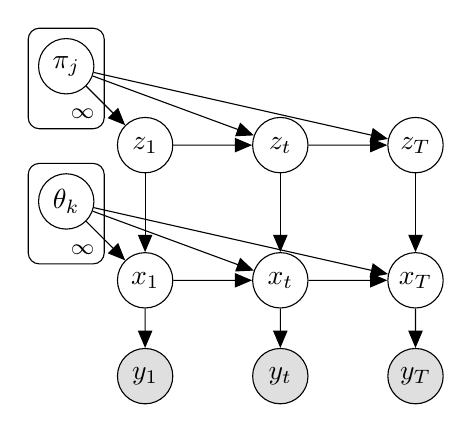
\begin{tikzpicture}[scale = 0.2]
        \node[latent] (pi_j) {$\pi_j$} ; 
        \node[latent, below = of pi_j] (theta_k) {$\theta_k$} ; 
        \node[latent, below right = 0.7cm of pi_j] (z_1) {$z_1$} ; %     
        \node[latent, right = of z_1] (z_t) {$z_t$} ; %                  
        \node[latent, right = of z_t] (z_T) {$z_T$} ; %                            
        \node[latent, below right = 0.7cm of theta_k] (x_1) {$x_1$} ; %     
        \node[latent, right = of x_1] (x_t) {$x_t$} ; %         
        \node[latent, right = of x_t] (x_T) {$x_T$} ; %                                  
        \node[obs, below = 0.5cm of x_1] (y_1) {$y_1$} ; %     
        \node[obs, right = of y_1] (y_t) {$y_t$} ; %         
        \node[obs, right = of y_t] (y_T) {$y_T$} ; %                                          
        %
        \plate{plate_pi} {(pi_j)} {$\infty$}; %
        \plate{plate_theta} {(theta_k)} {$\infty$}; %        
		%        
        \edge {pi_j} {z_1} ; %                               
        \edge {pi_j} {z_t} ; % 
        \edge {pi_j} {z_T} ; %         
        \edge {z_1} {z_t} ; %                               
        \edge {z_t} {z_T} ; %                                       
        \edge {theta_k} {x_1} ; %                               
        \edge {theta_k} {x_t} ; % 
        \edge {theta_k} {x_T} ; %         
        \edge {z_1} {x_1} ; % 
        \edge {z_t} {x_t} ; %         
        \edge {z_T} {x_T} ; %   
        \edge {x_1} {x_t}; %
        \edge {x_t} {x_T}; %                  
        \edge {x_1} {y_1} ; % 
        \edge {x_t} {y_t} ; %         
        \edge {x_T} {y_T} ; %                   
\end{tikzpicture}            
\end{figure}
\end{minipage}
\end{frame}

\section{Prior for HMM}

\begin{frame}
\frametitle{Keep Calm...}
\begin{minipage}{0.35\textwidth}
and put a prior...
\begin{itemize}
\item $\pi_j \sim DP(\alpha, \beta)$
\item But....
\end{itemize}

\end{minipage}
\begin{minipage}{0.55\textwidth}
\begin{figure}[!h]
      \centering
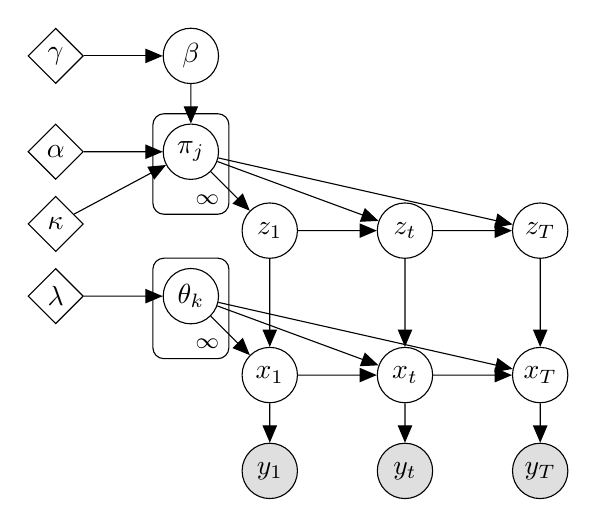
\begin{tikzpicture}[scale = 0.4]
        \node[det] (gamma) {$\gamma$} ; %
        \node[det, below = 0.5cm of gamma] (alpha) {$\alpha$}; 
        \node[det, below = 0.2cm of alpha] (kappa) {$\kappa$};       
        \node[det, below = 0.2cm of kappa] (lambda) {$\lambda$};       
        \node[latent, right = of gamma] (beta) {$\beta$} ; %                
        \node[latent, right = of alpha] (pi_j) {$\pi_j$} ; 
        \node[latent, right = of lambda] (theta_k) {$\theta_k$} ; 
        \node[latent, below right = 0.7cm of pi_j] (z_1) {$z_1$} ; %     
        \node[latent, right = of z_1] (z_t) {$z_t$} ; %                  
        \node[latent, right = of z_t] (z_T) {$z_T$} ; %                            
        \node[latent, below right = 0.7cm of theta_k] (x_1) {$x_1$} ; %     
        \node[latent, right = of x_1] (x_t) {$x_t$} ; %         
        \node[latent, right = of x_t] (x_T) {$x_T$} ; %                                  
        \node[obs, below = 0.5cm of x_1] (y_1) {$y_1$} ; %     
        \node[obs, right = of y_1] (y_t) {$y_t$} ; %         
        \node[obs, right = of y_t] (y_T) {$y_T$} ; %                                          
        %
        \plate{plate_pi} {(pi_j)} {$\infty$}; %
        \plate{plate_theta} {(theta_k)} {$\infty$}; %        
		%        
        \edge {gamma} {beta} ; %       
        \edge {beta} {pi_j} ; %               
        \edge {alpha} {pi_j} ; %                       
        \edge {kappa} {pi_j} ; %                       
        \edge {lambda} {theta_k} ; %                               
        \edge {pi_j} {z_1} ; %                               
        \edge {pi_j} {z_t} ; % 
        \edge {pi_j} {z_T} ; %         
        \edge {z_1} {z_t} ; %                               
        \edge {z_t} {z_T} ; %                                       
        \edge {theta_k} {x_1} ; %                               
        \edge {theta_k} {x_t} ; % 
        \edge {theta_k} {x_T} ; %         
        \edge {z_1} {x_1} ; % 
        \edge {z_t} {x_t} ; %         
        \edge {z_T} {x_T} ; %   
        \edge {x_1} {x_t}; %
        \edge {x_t} {x_T}; %                  
        \edge {x_1} {y_1} ; % 
        \edge {x_t} {y_t} ; %         
        \edge {x_T} {y_T} ; %                   
\end{tikzpicture}            
\end{figure}
\end{minipage}
\end{frame}


\begin{frame}
\frametitle{What does HDP mean in HMM?}
\begin{minipage}{0.35\textwidth}
Restaurant Analogy?
\begin{itemize}
\item Global Dish Menu?
\item Local Dish Menu?
\item Restaurant?
\item Dish?
\item Customer?
\end{itemize}
Better Analogy?
\end{minipage}
\begin{minipage}{0.55\textwidth}
\begin{figure}[!h]
      \centering
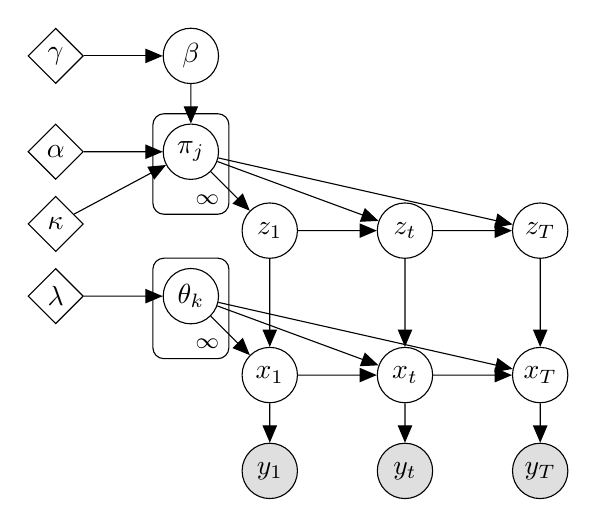
\begin{tikzpicture}[scale = 0.4]
        \node[det] (gamma) {$\gamma$} ; %
        \node[det, below = 0.5cm of gamma] (alpha) {$\alpha$}; 
        \node[det, below = 0.2cm of alpha] (kappa) {$\kappa$};       
        \node[det, below = 0.2cm of kappa] (lambda) {$\lambda$};       
        \node[latent, right = of gamma] (beta) {$\beta$} ; %                
        \node[latent, right = of alpha] (pi_j) {$\pi_j$} ; 
        \node[latent, right = of lambda] (theta_k) {$\theta_k$} ; 
        \node[latent, below right = 0.7cm of pi_j] (z_1) {$z_1$} ; %     
        \node[latent, right = of z_1] (z_t) {$z_t$} ; %                  
        \node[latent, right = of z_t] (z_T) {$z_T$} ; %                            
        \node[latent, below right = 0.7cm of theta_k] (x_1) {$x_1$} ; %     
        \node[latent, right = of x_1] (x_t) {$x_t$} ; %         
        \node[latent, right = of x_t] (x_T) {$x_T$} ; %                                  
        \node[obs, below = 0.5cm of x_1] (y_1) {$y_1$} ; %     
        \node[obs, right = of y_1] (y_t) {$y_t$} ; %         
        \node[obs, right = of y_t] (y_T) {$y_T$} ; %                                          
        %
        \plate{plate_pi} {(pi_j)} {$\infty$}; %
        \plate{plate_theta} {(theta_k)} {$\infty$}; %        
		%        
        \edge {gamma} {beta} ; %       
        \edge {beta} {pi_j} ; %               
        \edge {alpha} {pi_j} ; %                       
        \edge {kappa} {pi_j} ; %                       
        \edge {lambda} {theta_k} ; %                               
        \edge {pi_j} {z_1} ; %                               
        \edge {pi_j} {z_t} ; % 
        \edge {pi_j} {z_T} ; %         
        \edge {z_1} {z_t} ; %                               
        \edge {z_t} {z_T} ; %                                       
        \edge {theta_k} {x_1} ; %                               
        \edge {theta_k} {x_t} ; % 
        \edge {theta_k} {x_T} ; %         
        \edge {z_1} {x_1} ; % 
        \edge {z_t} {x_t} ; %         
        \edge {z_T} {x_T} ; %   
        \edge {x_1} {x_t}; %
        \edge {x_t} {x_T}; %                  
        \edge {x_1} {y_1} ; % 
        \edge {x_t} {y_t} ; %         
        \edge {x_T} {y_T} ; %                   
\end{tikzpicture}            
\end{figure}
\end{minipage}
\end{frame}

\begin{frame}
\frametitle{HDP in HMM: Mario's Warp Pipe Process}
\begin{figure}
\includegraphics[width=1\linewidth]{"./plot/mario_pipe"}
\end{figure}
\end{frame}

\begin{frame}
\frametitle{HDP in SLDS: Inference Overview}
Need to sample $(\bz, \beta, \bPi)$ and $(\bx, \bTheta)$ jointly:
\begin{itemize}
\item Sample $\bz, \beta, \bPi | \bTheta, \bx$
\begin{enumerate}
\item Sample $\bz \sim p(\bz | \bPi, \bTheta, \bx)$
\begin{itemize}
\item In contrast to conditional sampler in original HDP \\
 $p(z_t = k| \bz_{(-t)}, \beta) = p(z_t = k| \by)f(y_t|\by_{-(t)})$
\item efficiently algorithm available for Markov Model\\
(Forward-backward Message Passing)
\end{itemize}
\item Sample $\beta, \pi_k$ through standard CRF:
\begin{itemize}
\item $\beta | \bz \sim Dir(\bm, \gamma)$
\item $\pi_k | \beta, \bz \sim Dir(\alpha \beta_k + n_k)$
\end{itemize}
\end{enumerate}
\item Sample $\bx, \bTheta | \bz, \beta, \bPi$
\end{itemize}

\end{frame}



%%% Begin Will Section here
\section{Switching Linear Dynamical Systems}
\begin{frame}
\frametitle{Linear Dynamical Systems}

For times $t=1\ldots T$, we are given data $y_t\in\mathbb{R}^n$. We assume $y_t$ is a noise observation of a hidden, continuous state $x_t\in\mathbb{R}^d$, with $d\geq n$, and that $x_t$ is a markov chain. The probability model is:
\begin{align*}
x_t|x_{t-1}&\sim\mathcal{N}(Ax_{t-1}+B,\Sigma)\\
y_t|x_t&\sim\mathcal{N}(Cx_t,R)
\end{align*}
We assume $C$ is known.

\end{frame}

\begin{frame}
\frametitle{Switching Linear Dynamical Systems}

We now assume at each time $t$ there is a hidden mode indexed by $z_t\in\{1,\ldots,K\}$ that determines the dynamical regime. The probability model is:
\begin{align*}
x_t|x_{t-1},z_t&\sim\mathcal{N}(A^{(z_t)}x_{t-1}+B^{(z_t)},\Sigma^{(z_t)})\\
y_t|x_t&\sim\mathcal{N}(Cx_t,R)
\end{align*}
In the standard SLDS, $K<\infty$. In the HDP-HMM-SLDS, $K=\infty$.
\end{frame}

\begin{frame}
\frametitle{Algorithms for Inference}
\begin{itemize}
\item Conditional on known dynamical parameters $A,B,\Sigma$ and $z_{1:T}$, the hidden states $x_{1:T}$ are obtained via a \textbf{Kalman sampler}.
\item Conditional on known hidden states $x_{1:T}$, the hidden modes $z_{1:T}$ are obtained via the \textbf{Forward-Backward} (sampling) algorithm.
\item Conditional on known $x_{1:T},z_{1:T}$, the dynamical parameters are obtained via \textbf{multivariate linear regressions} for each of the modes.
\end{itemize}
\end{frame}

\begin{frame}
\begin{figure}
  \centering
  \includegraphics[width = 1\linewidth]{"./plot/lds/01_projectile_known"}
\end{figure}
\end{frame}

\begin{frame}
\begin{figure}
  \centering
  \includegraphics[width = 1\linewidth]{"./plot/lds/02_projectile_unknown"}
\end{figure}
\end{frame}

\begin{frame}
\begin{figure}
  \centering
  \includegraphics[width = 1\linewidth]{"./plot/lds/03_harmonic_known"}
\end{figure}
\end{frame}

\begin{frame}
\begin{figure}
  \centering
  \includegraphics[width = 1\linewidth]{"./plot/lds/04_harmonic_unknown"}
\end{figure}
\end{frame}

\begin{frame}
\frametitle{Lessons Learned}
\begin{enumerate}
\item Kalman sampler great when dynamical parameters known.
\item When dynamical parameters unknown, choice of prior is crucial.
\item ``Uninformative'' hyperparameters didn't work. Need regularization.
\item Non-stationary time series present problems for empirical bayes.
\item Higher dimensional state space is more flexible but may overfit.
\end{enumerate}
\end{frame}

\end{document}